\documentclass[12pt,twoside,a4paper]{article}
\usepackage[utf8]{inputenc} \usepackage[T1]{fontenc} \usepackage{graphicx}

\usepackage{listings}
\lstloadlanguages{Matlab,C}
\lstset{% general command to set parameter(s)
basicstyle=\sffamily\footnotesize, % print whole listing small
keywordstyle=\sffamily\footnotesize\bfseries, % ubold black keywords
identifierstyle=, % nothing happens
commentstyle=\sffamily\footnotesize\slshape, % green comments
stringstyle=\sffamily\footnotesize, % typewriter type for strings
showstringspaces=false, % no special string spaces
%numbers=left,
numberstyle=\sffamily\footnotesize,
stepnumber=1,
numbersep=10pt,
showspaces=false,
showtabs=false,
%frame=lines,
morecomment=[l]{\%},
float=htbp,
numberbychapter=true
}
\setlength\parindent{0pt} 
\begin{document}

Subtraktion von binären Zahlen

Drei Schritte zu Subtraktion:

Das Einerkomplement
Das Zweierkomplement
Die Subtraktion von Dualzahlen

Einerkomplement

Was ist das Komplement von Dualzahlen? Man bildet das sogenannte Einerkomplement, indem man jede Zahl durch ihr Gegenteil ersetzt, also die 0 durch die 1 und die 1 durch die 0.\\

01011010 wird zu 10100101\\
11101101 wird zu 00010010\\

\paragraph{Das Zweierkomplement}

Das Zweierkomplement entspricht dem Einerkomplement, nur wird zusätzlich noch 00000001 addiert.

01011010 wird im Einerkomplement zu 10100101 im Zweierkomplement zu 10100110
11101101 wird im Einerkomplement zu 00010010 im Zweierkomplement zu 00010011

\paragraph{Konvertierung von Festkommazahlen Dez zu Bin}

10,2 \\
\\

Vorkommastelle
10 = 1010

Nachkommastelle\\
\emph{0,2} * 2 = 0,4 + 0 \emph{MSB} \\ 
0,4 * 2 = 0,8 + 0\\
0,8 * 2 = 0,6 + 1\\
0,6 * 2 = \emph{0,2} + 1 \emph{LSB} \\ 

Sobald es sich wiederholt kann aufgehört werden.\\
0, 2 = 0,0011\\
10,2 = 1010,00110011 $\approx$ 0,19921875
\\
$\Longrightarrow$ Eine Abweichung von  -0,00078125
\\
\paragraph{Konvertierung von Fließkommazahlen Dez zu Bin}
18,4$_{10}$ \\


18$_{10}$  = 10010$_{2}}$ \\
0,4$_{10}$ = 0,011$_{2}}$ \\


\section{mov vs. ldr}
\begin{center}
  \begin{tabular}{ | l | l | l |}
    \hline
    ldr & mov  & Funktion\\ \hline
    r1, [r2] & r1, r2 & speichere Wert von r2 in r1 \\ 
    r1, =255 & r1, #255 & speichere 255 in r1 \\ 
    Bewegt Speicher/Register & Bewegt Register & - \\
    32-Bit & 8-Bit & - \\
    \hline
  \end{tabular}
\end{center}




\paragraph{Die Subtraktion von Dualzahlen}

Der Satz lautet: Die Subtraktion von 2 Zahlen erfolgt durch die Addition des Zweierkomplementes. Als konkretes Beispiel nehmen wir dazu die Rechnung 14-9=5.

9 ist im Dualsystem 00001001.
Das Einerkomplement zu 00001001 ist 11110110.
Das Zweierkomplement 11110111.
Dies addieren wir nun zu 14 also 00001110.

\begin{lstlisting}
   00001110 
  +11110111 
   ========
   00000101
\end{lstlisting}

Auch hier wäre die richtige Zahl eigentlich 00000101 Übertrag 1, da wir den Übertrag jedoch nicht speichern können, bleiben wir bei 00000101 was ja der Dezimalzahl 5 entspricht.

\paragraph{Little-/Bigendian}
\begin{figure}[ht!]
\centering
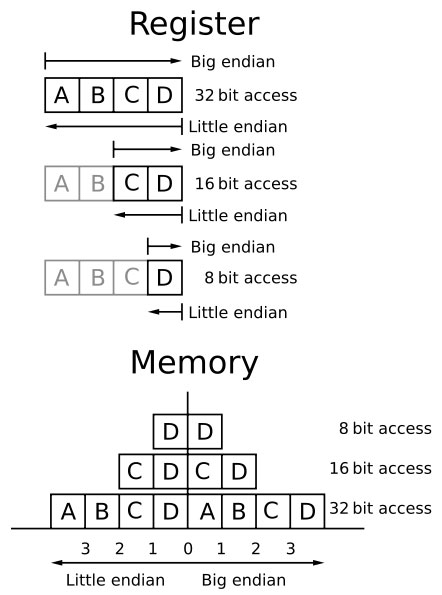
\includegraphics[width=90mm]{big-endian_und_little-endian.jpg}
\caption{A simple caption \label{overflow}}
\end{figure}

\section*{Assemblerbefehle}
\begin{lstlisting}
AREA MyCommonBlock, COMMON, ALIGN = 10 ; Read-Write-Data
MyCommonBlock bezeichnet die Anfangsadresse des Speicherblocks
COMMON: vom Linker mit Nullen initialisierter Speicherbereich
Alignment mit 2^{10} erzeugt eine Blockgrenze bzw. –anfang mit n * 1024

mov r0, #0x21
Lade #0x21 in Register R0:
R0
00000021
\end{lstlisting} 

\subparagraph{Angabe negativer Konstanten}
mov r1, #-10

\paragraph{Speicherreservierung}
\begin{lstlisting}
DCB  8 Bit
DCW 16 Bit
DCD 32 Bit
\end{lstlisting}

\newpage
\section*{Lösungen für Tests}
% !TEX root = rmp_lernzettel.tex


\section{Lösung für Test 1:}
\subsection{}
Wie lautet die Hexadezimalzahl zur Binärzahl?
\paragraph{Lösung}
\begin{lstlisting}
1001 1101 1010
\end{lstlisting}
\begin{lstlisting}
   9    D   10 
\end{lstlisting}
\subsection{}
Wie lautet die Binärzahl zur Dezimalzahl 97
\paragraph{Lösung}
0110 0001
\paragraph{Erklärung}
1*64 + 1*32 + 1*1
\subsection{} 
Addieren Die nebenstehende 8-Bit Binärzahlen:\\
\\
Ist das Carry-Flag gesetzt:\\
Ist das Overflow-Flag gesetzt:
\begin{lstlisting}
 0111 1111
+1011 0011 
\end{lstlisting}
\paragraph{Lösung}
\begin{lstlisting}
   0111 1111
  +1011 0011
------------
U 11111 1110
------------
   0011 0010
\end{lstlisting}
Carry-Flag: 	ja\\
Overflow-Flag:	nein\\

\paragraph{Erklärung}
Das Carry-Flag ist gesetzt dar der hinterste Übertrag auf 1 gesetzt ist.\\
Das Overflow-Flag ist nicht gesetzt dar der hinterste und der vorhinterste Übertrag in Xor-Verbindung 0 ergibt.\\

\subsection{}

Geben Sie den Dezimalwert zur Hexadezimalzahl 7D an.

\paragraph{Lösung}
125

\paragraph{Erklärung}
\begin{lstlisting}
Hex $\rightarrow$          7 |       D\\
Bin $\rightarrow$ 0  1  1  1 | 1 1 0 1\\
Dez $\rightarrow$ / 64 32 16 | 8 4 / 1 = 125\\
\end{lstlisting}

\subsection{}

Wie lautet die 8-Bit-Zweierkompliment-Darstellung zur Dezimal -97?

\paragraph{Lösung}
\begin{lstlisting}
                 -97 = 1001 1111
Zweierkompliment: 97 = 0110 0001
\end{lstlisting}


\paragraph{Erklärung}
-128 + 16 + 8 + 4 + 2 + 1 = -97

$\rightarrow$ Zweierkompliment = Binär invertieren + 0000 0001

\subsection{}

Woran erkennt man bei der Subtraktion zweier Vorzeichenbehafteter Zahlen, ob das berechnete Ergebnis falsch ist?

\paragraph{Lösung}
Overflow-Flag:\\
=1 $\rightarrow$ flasch\\
=0 $\rightarrow$ richtig

\paragraph{Erklärung}
s.o.
\subsection{}
Das Datenfeld...


\subsection{}

Ab Adresse 0x1004 steht folgendes im Speciher (hex.) little endian:
\begin{lstlisting}
14 21 32 A3 A7 F3 FA
\end{lstlisting}
Was steht in r1 nach folgender Sequenz?

\begin{lstlisting}
mov	r0, #0x1006
ldrh	r1, [r0]
\end{lstlisting}

\paragraph{Lösung}



\newpage
% !TEX root = rmp_lernzettel.tex

\section{Lösung für Test 2:}
\subsection{}
\begin{lstlisting}
Bytefeld 	DCB 	11,'B', 0xB, 0b01000010
\end{lstlisting}

a)
\begin{lstlisting}
Bytefeld 	0B, 42, 11, 42
\end{lstlisting}
 
b)
\begin{lstlisting}
ldr r1, =Bytefeld
ldrb r0, r1 
\end{lstlisting} 
 
c)
\begin{lstlisting}
0x11, B
\end{lstlisting} 

\subsection{}
\begin{lstlisting}
ALIGN 4
mov r0, 0xAB
\end{lstlisting} 

\subsection{}
\begin{lstlisting}
ldr r0, 0x1256ABCD
\end{lstlisting} 

\subsection{}
\begin{lstlisting}
bgt
\end{lstlisting} 

\subsection{}
\begin{lstlisting}
bgt
\end{lstlisting} 
 
\subsection{}
Aufgabe:\\
Die \textbf{vorzeichenlose} Zahl in r0 soll durch 4 geteilt werden. Das Ergebnis soll in r1 stehen.\\
Geben Sie den Befehl an:\\


\paragraph*{Lösung:}

\begin{lstlisting}
MOV r0,r1,ASR #2
\end{lstlisting}


\paragraph*{Erklärung:}
Eine Verschiebeoperation nach \textbf{links} um 1 Bit entspricht der \textbf{Multiplikation} mit 2 \\
und eine Verschiebeoperation nach \textbf{rechts} um 1 Bit entspricht der \textbf{Division} mit 2. \\
Warum \# 2 statt 4? \# 1 $\rightarrow$ x $\div$ 2; \# 2 $\rightarrow$ x $\div$ 2 $\div$ 2 $\rightarrow$ x $\div$ 4 


\paragraph*{Nachschlagen:}
Kapitel 8.5.5

\subsection{}
Aufgabe:\\
Das Datenfeld Var1 beginne bei Adresse 0x2000. Welcher Wert (hex.) vsteht nach Ausführung des Befehls in r0?\\

\begin{lstlisting}
Var1 	DCB 	10, 'A', 0xA, '1'

		ldr r0, =Var1
\end{lstlisting}

\paragraph*{Lösung}
r0 = 0x2000

\paragraph*{Erklärung:}
Lade die Adresse von Var1 in r0. 


\paragraph*{Nachschlagen:}
Kapitel 7.5.3

\subsection{}
Das Datenfeld Tab beginne bei Adresse 0x2000. Geben Sie die Speicherinhalte (hex.) von Adresse 0x2000 - 0x2003 an?\\
\begin{lstlisting}
Var1 	DCB 	0x10, 'A', 10, '1'
\end{lstlisting}

\paragraph*{Lösung}
0x2000: 41 0A 31 10 \\


\paragraph*{Erklärung:}
0x10 $\rightarrow$ Hexadezimal $\rightarrow$ 10\\
'A' $\rightarrow$ ASCII $\rightarrow$ 41\\
10 $\rightarrow$ Hexadezimal $\rightarrow$ A\\
'1' $\rightarrow$ ASCII $\rightarrow$ 41\\

\paragraph*{Nachschlagen:}
Kapitel 7.4.3 Folie 18 $\rightarrow$ Wie werden die Sachen gespeichert?\\
Kapitel 6.4 $\rightarrow$ Reihenfolge im Speicher\\

\subsection{}
Folgendes Datenfeld sei gegeben:
\begin{lstlisting}
Var1 	DCD 	0x10, 0xAA12
\end{lstlisting}
Geben Sie die Assemblerbefehle an, um das \underline{erste Datenwort} des Feldes Var1 nach r1 zu kopieren

\paragraph*{Lösung:}
\begin{lstlisting}
ldr r0, =Var1 ; Arraystartadresse laden 
ldr r1, [r0] ; Erstes Element des Arrays
\end{lstlisting}
\paragraph*{Erklärung:}
Warum nicht mov?\\
mov kopiert nur ein Datenwort Syntax: MOV <wohin>, <woher,was> $\rightarrow$ Daten > \\
Nachschlagen von MOV: Kapitel 6.9.3\\
\paragraph*{Nachschlagen:}
Kapitel 7.5.3
Kapitel 7.7.3


\subsection{}
Was steht in r0 nach folgendem Befehl (hex.)?
\begin{lstlisting}
ldr 		r0, =0x1234ABCD
\end{lstlisting}


\paragraph*{Lösung:}
r0 = 0x1234ABCD

\paragraph*{Erklärung:} 
Wenn nach '=' ein Hexwert kommt dann speichere den Wert. Wenn Variable, dann speichere die Adresse.\\
Auch hier würde mov nicht funktionieren, da 0x1234ABCD > 8 Bit\\


\paragraph*{Nachschlagen:}
\url{http://www.keil.com/support/man/docs/armasm/armasm_dom1361289875065.htm} \\
\url{https://www.raspberrypi.org/forums/viewtopic.php?&t=16528}

\subsection{}
In welchem Wertebereich muss r0 liegen, damit ein Sprung nach LOOP erfolgt? (dezimal oder hex.)
\begin{lstlisting}
mov		r1, #-15
cmp		r0, r1
bge		LOOP	;if greater or equal
\end{lstlisting}

Größer oder gleich:\\
Kleiner oder gleich:\\

\paragraph*{Lösung:}
Größer oder gleich: -15\\
Kleiner oder gleich: 255\\

\paragraph*{Erklärung:}
greater or equal $\rightarrow$ r1 muss >= -15 
mov r1 $\rightarrow$ 8-Bit $\rightarrow$ 1 muss <= 255

\paragraph*{Nachschlagen:}
bge $\rightarrow$ Kapitel 8.3.5

\subsection{}
Was steht in r0 nach folgender Befehlssequenz (hex.)?
\begin{lstlisting}
ldr		r1, =0xFFFFFF87
mov		r0, #0x78
and		r0, r1
\end{lstlisting}

\paragraph*{Lösung:}

\begin{lstlisting}
r1 1111 1111 1111 1111 1111 1111 1000 0111
r0 0000 0000 0000 0000 0000 0000 0111 1000
------------------------------------------
r0 0000 0000 0000 0000 0000 0000 0000 0000
\end{lstlisting}

\paragraph*{Erklärung:}
logisches UND nur wenn gleiche Werte in r1 und r0 stehen $\rightarrow$ 1

\paragraph*{Nachschlagen:}
Kapitel 8.4.3
\newpage
% !TEX root = rmp_lernzettel.tex

\section{Lösung für Test 3:}
Gegeben ist folgendes Programmfragment (für die Aufgaben 1-3):
\begin{lstlisting}
		AREA MyData, DATA, align = 8
VarA			DCD		0x17, 17, 0xA, 'A'
VarB			DCB		33, -1, 0x10, 0x20, 0x30, 'a', '1'
\end{lstlisting}
\subsection{}
\begin{lstlisting}
ldr 	r0,= VarA	; Lade den Anfang von VarA in r0
ldr 	r1, [r0]	; Lade das erste Elemente von VarA in r1
ldr 	r2, [r0 #4]	; Lade das zweite Element von VarA in r2 (pre increment)
adds	r1, r1, r2	; Addiere r1 und r2 und speichere das Ergebnis in r1
\end{lstlisting}

\subsection{}
\begin{lstlisting}
VarB = 0x2010
VarA = 0x2000
VarB - VarA = 0x2010 - 0x2000 = 0x0010	; Anfangsadressen werden subtrahiert
\end{lstlisting}

\subsection{}
  \begin{tabular}{ | c | c | c | c | c | c |}
    0x2000 & 0x2001  & 0x2002 & 0x2003 & 0x2004 & 0x2005 \\
    0x17 & 00  & 00 & 00 & 0x11 & 00 \\
  \end{tabular}\\
Zu Beachten: align = 8 $\rightarrow$ Es wird auf 8 Byte aufgefüllt.

\subsection{}
\begin{lstlisting}
bl MyProg
\end{lstlisting}
bl (branch link) springt bedingungslos.

\subsection{}
Speichert die Rücksprungsstelle.
\begin{lstlisting}
r14
\end{lstlisting}.
\paragraph*{Nachschlagen:}
Kapitel 10.1.3.2 

\subsection{}
Der Stackpointer zeigt uns an welcher Stelle wir uns im Stack befinden.
\begin{lstlisting}
r13
\end{lstlisting}

\subsection{}
push{} fügt etwas dem Stack hinzu.
sp (Stackpointer) wird ums eins verringert.
\paragraph*{Nachschlagen:}
Kapitel 9.2

\subsection{}
\begin{lstlisting}
push 	{fp, lr}
mov 	fp, sp
push 	{r1 - r4}	; 8-align -> gerade Anzahl Registern
pop 	{r1 - r4}	; 8-align -> gerade Anzahl Registern
pop		{fp, lr}
bx		lr
\end{lstlisting}
\paragraph*{Nachschlagen:}
Kapitel 9.3.1

\subsection{}
\begin{lstlisting}
push 	{r1 - r4}
bl
...
add		sp, #16
\end{lstlisting}

\subsection{}
Vereinfacht Zugriff auf lokale Daten.
\begin{lstlisting}
r11
\end{lstlisting}
\paragraph*{Nachschlagen:}
Kapitel 10.2.3.1

\end{document}
